
\chapter{Machine Learning} \label{ML}

\section{Introduction}

" We use AI so much that we have stopped thinking of it as AI, ”  says Nello Cristianini,  professor of artificial  intelligence at the university of Bristol.

Nowadays we make many decisions based on our past experiences,  or based on what we expect in the future, either way we sure take a lot of bad decisions and make a lot of mistakes, Machines ( computers ) Can be a powerful tool for this type of tasks with higher prediction ( about future ) and better accuracy, and that's when machine learning comes, which is actually a process  that teaches computers to tackle enormous amounts of data, and pull out patterns that can represent a model able to  make decisions, but these models are still yet in need of human supervision to evaluate it, and help it overcome the complexities hidden in data .

In this chapter we will first define supervised learning and presents one of the powerful application of such type of learning ( supervised ) SVM algorithm ( support vector machine )  and nearest neighbor algorithm, and then define the second type unsupervised learning   with a review K-means algorithm, these algorithm  proved  to be accurate and robust  for our HGR system as it's going to be shown in  chapter  [\ref{hgr}]

\section{Supervised machine learning}

The goal of supervised learning is to approximate the mapping function so well that when we have new input data (x) then we can predict the output variables (Y) for that data. When (Y) categorical,the problem is known as <<classification>>, and when (Y) represents floating values, in this case the process is knows as <<regression>> .

Some popular examples of supervised machine learning algorithms are:
Linear regression for regression problems.
Support vector machines for classification and regression problems.

\section{Support vector machines (SVM) }\label{sec:svm}
It's a supervised machine learning algorithm, the intuition  behind it  is to find a hyperplane that best divides a dataset into two classes, a good separation is achieved by the hyperplane, that has the largest distance to the nearest training-data point of any class (so-called functional margin), since in general the larger the margin the lower the  error of the classifier.

But first let us define what is a hyperplan;  it's a line that  linearly separates and classifies a set of data. As the fig \ref{122} shows, our hyperplan here is the line that separate the green data from red data .

\begin{figure}[H]
\centering
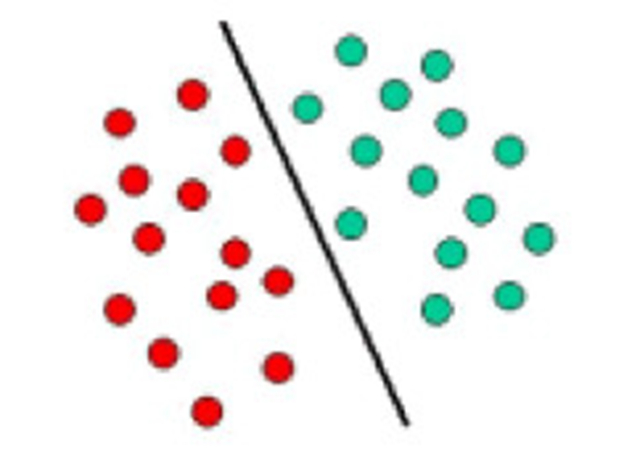
\includegraphics[width=0.3\textwidth]{img/svm1.png}
\caption{example of linear Hyperplan seperating Green data from Red data }
\label{122}
\end{figure}


The above is a classic example of a linear classifier, the hyperplan should be optimal for our classification task which turns to maximize the margin, which is basically the distance between the hyperplane,  and the nearest data point from either set,  the greater this margin is the better for the classifier to make  describe data .But data is not always linearly separable as in real world problems we usually deal with linearly non separable kind of data as shown  in the figure \ref{123 }, 

\begin{figure}[H]
\centering
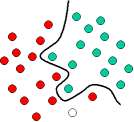
\includegraphics[width=0.3\textwidth]{img/svm2.png}
\caption{Non linear Example of data  }
\label{123 }
\end{figure}
For this reason, it was proposed that the original finite-dimensional space be mapped into a much higher-dimensional space, presumably making the separation easier in that space, this is often called the kernel trick and it uses a set of mathematical functions (kernels). Using a higher dimension we can  linearly  seperate the data, thus, instead of constructing the complex curve (left schematic), all we have to do is to find an optimal line that can separate ( right schematic ) .



\begin{figure}[H]
\centering
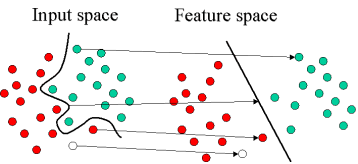
\includegraphics[width=0.5\textwidth]{img/SVMIntro3.png}
\caption{Non linear separated using kernel (higher dimension) }
\label{124 }
\end{figure}


\subsection{Hard-Margin SVM}
The SVM technique is a classifier that finds a hyperplane or a function $g(x) = {\omega}^T +  b$   that correctly separates two classes with a maximum margin.The figure below shows a separating hyperplane corresponding to a hard-margin SVM (also called a linear SVM).

\begin{figure}[H]
\centering
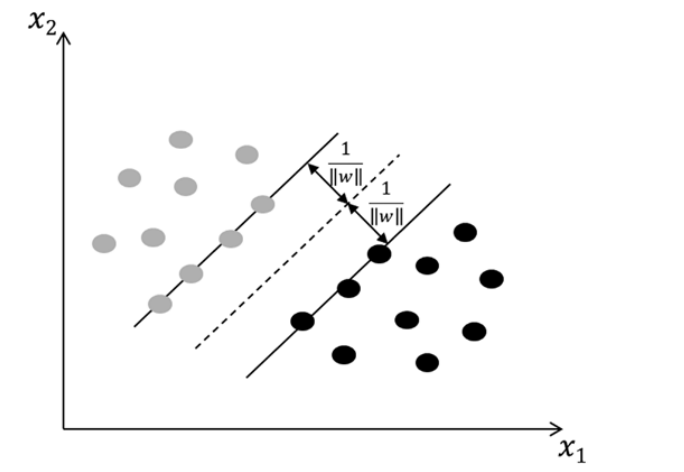
\includegraphics[width=0.5\textwidth]{img/hardmargin.PNG}
\caption{ Hard-maximum-margin separating hyperplane. }
\label{125 }
\end{figure}


\subsection{Soft-Margin SVM}
SVM is classifying most of the data correctly, while allowing the model to misclassify a few points in the vicinity of the separating boundary

\begin{figure}[H]
\centering
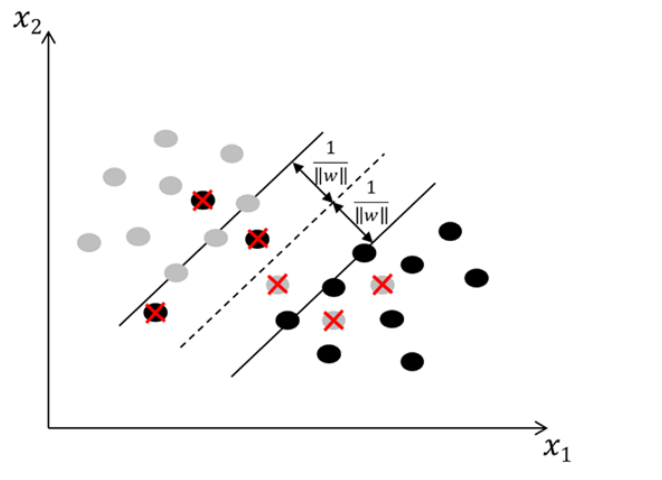
\includegraphics[width=0.5\textwidth]{img/softmargin.PNG}
\caption{  A few misclassifications, as part of soft-margin SVM . }
\label{126 }
\end{figure}


\subsection{Kernels}

In most Real cases, the optimal boundary is not linear,  the idea of NON linear SVM is to map the data into a higher dimensional space where data can linearly separable, this is often called the kernel trick . A kernel should be a Hermitian and positive semidefinite matrix and needs to satisfy Mercer’s theorem, which translates into evaluating the kernel or Gram matrix on all pairs of data points as positive and semi-definite, forming:

$K(\small{x,u})=\sum\limits_{r} \phi(x)\phi(u) $ .

where $\phi(x) $ belongs to the Hilbert space.
\newline
$$\int \int K(x,u) g(x) g(u) du dx \geq 0 \ \ \ \ \forall g(x) , \ where \int g^2(x) dx < +\infty$$
\\
\newline 
Some popular kernel functions include: 


\begin{itemize}

  \item  Linear kernel  : 
  \begin{align*}
  \mathlarger {K(x,u)=  x^{T}.u  }
   \end{align*}
  \item Polynomial function: 
  \begin{align*}
  K(x,u)=(ax^{T}u + c)^{q} ,\, q>0.
  \end{align*}
  \item Gaussian radial basis function (RBF): 
\begin{align*} 
 K(x,u) = e^{\mathlarger{\frac{\mathbf{-\| x -  u\|^2}}{\mathbf{\sigma^2} } }}
\end{align*}
   
  \item  Hyperbolic tangent (sigmoid):
    \begin{equation}
      K(\mathbf x, \mathbf u) = \tanh(\mathbf {\beta} \mathbf x^{T} \mathbf u - \mathbf{\delta})^p
    \end{equation}
    
    \item Laplacian radial basis function : 
    
    \begin{align*} 
      K(x,u) = e^{\mathlarger{\frac{-\| x -  u\|}{\sigma} } }
     \end{align*}
    
\end{itemize}

Kernel selection is heavily dependent on the data specifics. For instance, the linear kernel the simplest
of all is useful in large sparse data vectors. However, it ranks behind the polynomial kernel, which avoids zeroing the Hessian. \\The polynomial kernel is widely used in image processing, the Gaussian and Laplace RBFs are general-purpose kernels that are mostly applied in the absence of prior knowledge. \\A kernel matrix that ends up being diagonal indicates that the feature space is redundant and that another kernel should be tried after feature reduction.\\\textbf{
Note} that when kernels are used to transform the feature vectors from input space to kernel space for linearly non-separable datasets, the kernel matrix computation requires massive memory and computational resources for big data . 



\section{Nearest neighbour based classifiers}

One of the simplest decision procedures that can be used for classification is the
nearest neighbour (NN) rule. It classifies a sample based on the category of its nearest
neighbour.When large samples are involved,it can be shown that this rule has a
probability of error which is less than twice the optimum error
—hence there is less
than twice the probability of error compared to any other decision rule. The nearest
neighbour based classifiers use some or all the patterns available in the training set
to classify a test pattern. These classifiers essentially involve finding the similarity
between the test pattern and every pattern in the training set.

\subsection{Nearest neighbour algorithm}
The nearest neighbour algorithm assigns to a test pattern the class label of its closest
neighbour

% Insert the algorith

\begin{algorithm}[H]
\SetAlgoLined

 Initialization\;
 $ A=(X_{1},\omega_{1}),(X_{2},\omega_{2}),....,(X_{n},\omega_{n}) \ // A\ is\ the\ set\ of\ N\ training\ pattern $\\
 
 
$ //where\  X_{i}\ is\ of\ dimension\ n\ and\  \omega_{i}\ is\ the\ class\ label\ of\ the\ i^{th}\ pattern $\\
 
 
 $d(u,x) = \sqrt{\sum_{k=0}^{N} (u_{i}-x_{i})^{2}}  // \ Euclidean\ distance\ measure $\\ 

 \While{ i \neq N }{ // N samples
 
  d(X_{t},X_{i}) = min {D(X_{t},X_{i})}\; 
 
 }
 
 $ X_{t} = \omega_{k} $ \\
 
 $ pattern\ X_{t}\ is\ assigned\ to\ a\ class\ \omega_{k}\ associated\ with\  X_{k} $
 
 \caption{Algorithm for NN}
\end{algorithm}



\subsection{K-nearest neighbour (kNN) algorithm}
 the k-nearest neighbors algorithm (k-NN) is a non-parametric method used for classification and regression.  In both cases, the input consists of the k closest training examples in the feature space. The output depends on whether k-NN is used for classification or regression:
\begin{itemize}
\item In k-NN classification, the output is a class membership. An object is classified by a majority vote of its neighbors, with the object being assigned to the class most common among its k nearest neighbors (k is a positive integer, typically small). 
\item In k-NN regression, the output is the property value for the object, this value is the average of the values of its k nearest neighbors.
\end{itemize}

K-NN is a type of instance based learning, or lazy learning, where the function is only approximated locally and all computation is deferred until classification. The k-NN algorithm is among the simplest of all machine learning algorithms.\\ Both for classification and regression, it can be useful to assign weight to the contributions of the neighbors, so that the nearest neighbors contribute more to the average than the more distant ones. For example, a common weighting scheme consists in giving each neighbor a weight of 1/d, where d is the distance to the neighbor.\\ The neighbors are taken from a set of objects for which the class (for k-NN classification) or the object property value (for k-NN regression) is known. This can be thought of as the training set for the algorithm, though no explicit training step is required.



%%%%%%%%%%%%%%%%%%%%%%%%%
\section{Unsupervised learning}

In supervised learning, the aim is to learn a mapping from the input to
an output whose correct values are provided by a supervisor.\\
In unsupervised
learning, there is no such supervisor and we only have input data.
The aim is to find the regularities in the input, there is a structure to the
input space such that certain patterns occur more often than others, and we want to see what generally happens and what does not. In statistics, this is called density estimation.
One method for density estimation is clustering where the aim is to
find clusters or groupings of input.\\ 
Some popular examples of unsupervised learning algorithms are:


\begin{itemize}
  \item k-means for clustering problems.
  \item Apriori algorithm for association rule learning problems.
\end{itemize}


\section{ K-Means clustering }\label{kmeans}
K-means \cite{kmeans} is one of the simplest unsupervised learning algorithms that solve the well known clustering problem. \\ K-Means clustering intends to partition n objects into k clusters in which each object belongs to the cluster with the nearest mean. This method produces exactly k different clusters of greatest possible distinction. The best number of clusters k leading to the greatest separation (distance) is not known as a priori,  and must be computed from the data. The objective of K-Means clustering is to minimize total intra-cluster variance, or, the squared error function:
\begin{figure}[H]
\centering
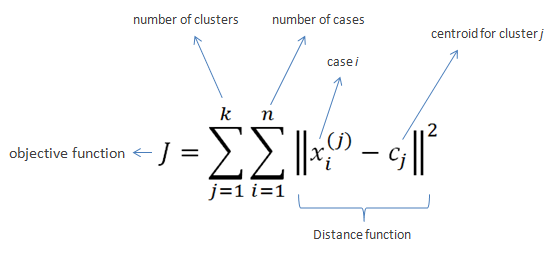
\includegraphics[width=0.7\textwidth]{img/ckmeans.png}
\end{figure}

 The algorithm as described by \cite{kmeans} starts with a random set of $k$ center-points ($\mu$). During each update step, all observations $x$ are assigned to their nearest center-point (see equation \ref{eqn:kmeans_assign_step}). In the standard algorithm, only one assignment to one center is possible. If multiple centers have the same distance to the observation, a random one would be chosen.

\begin{equation}
S_i^{(t)} = \big \{ x_p : \big \| x_p - \mu^{(t)}_i \big \|^2 \le \big \| x_p - \mu^{(t)}_j \big \|^2 \ \forall j, 1 \le j \le k \big\}
\label{eqn:kmeans_assign_step}
\end{equation}

Afterwards, the center-points are repositioned by calculating the mean of the assigned observations to the respective center-points (see \ref{eqn:kmeans_update_step}).

\begin{equation}
\mu^{(t+1)}_i = \frac{1}{|S^{(t)}_i|} \sum_{x_j \in S^{(t)}_i} x_j
\label{eqn:kmeans_update_step}
\end{equation}

The update process reoccurs until all observations remain at the assigned center-points and therefore the center-points would not be updated anymore.

\begin{algorithm}
\caption{Algorithm of cluster centroids initialization}

\begin{algorithmic}[1]

\Function{}{}

\State {\textbf{Input:} Data set $X = \{x^{(1)}, x^{(2)}, ..., x^{(m)} | c^{(i)} \in \mathbf{R}^n\}$}
\State {\textbf{Output:} Initial cluster centroids $\mu_{i=1, ..., k} \in \mathbf{R}^n$}
\State {Choose two samples $x^{(i)}$, $x^{(j})$ with largest distances as first two cluster centroids 
\\ \ \ \ \ \ $\mu_1 , \mu_2$ , $X \ =\ X\ -\ \{x^{(i)}, x^{(j)}\}$};

\For{$i=3, ... , k$ do }
\Comment{Choose other cluster centroids}
\State {Compute the sum of distance with all existing cluster centroids};
\State {$D^{(j)} = \sum_{t=1}^{i-1}{{\left \|x^{(j)}-\mu_t \right \|}^2}$};
\State {$X = X - x^{(j)}$};
\EndFor

\Return{$\mu_1, \mu_2, ..., \mu_k$ ;}
\EndFunction
\end{algorithmic}
\end{algorithm}


\section{Model selection } \label{ms}
Model selection is the process of choosing between different machine learning approaches,  or choosing between different hyperparameters or sets of features for the same machine learning approach  like in SVM kernels deciding between the RBF degrees and linear kernels.
The choice of the actual machine learning algorithm is less important than we'd think  there may be a "best" algorithm for a particular problem, but often its performance is not much better than other well performing approaches for that problem.


There may be certain qualities we look for in an model:

\begin{itemize}
\item Interpretable   can we see or understand why the model is making the decisions it makes?
\item Simple   easy to explain and understand
\item Accurate
\item Fast (to train and test)
\item Scalable (it can be applied to a large dataset)

\end{itemize}
Though there are generally trade offs among these qualities.\\in order to select a model from other models, we usually use one of the following approaches.\\\textbf{A Typical approach } is to take your data and split it randomly into a training set and a test set (e.g. a 70\%/30\% split). Then you train your model on the training set and see how it performs on the test set.\\The problem with this approach is that it results in an overly optimistic estimation of generalization if we tune our model's parameters with it,  so what we want to do instead is splitting the data is to not split it only into training and testing sets, but to also include a validation set. A typical ratio is 60\% training, 20\% validation, 20\% testing.

This way we can measure validation error instead of just measuring the test error .
We can use these errors   to identify what kind of problem we have if our model isn't performing well:

\begin{itemize}
\item If our training error is large and our validation/test set error is large, then we have a high bias (underfitting) problem.
\item If our training error is small and our validation/test set error is large, then we have a high variance (overfitting) problem.
\end{itemize}
As the figure \ref{fig:bias} explains : 

\begin{figure}[H]
\centering
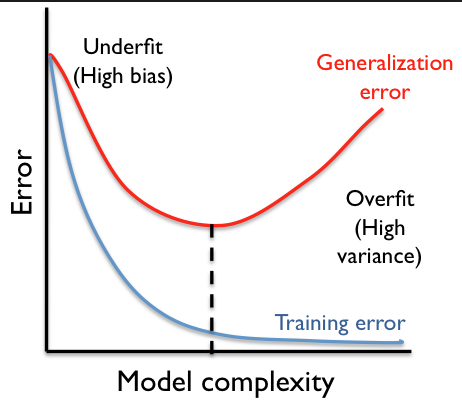
\includegraphics[width=0.5\textwidth]{img/model.png}
\caption{ bias / variance Tradeoff}
\label{fig:bias}
\end{figure}

Some ways of evaluating a model's performance on (some of)  known data are for \textbf{validation set } to pick  the best model you can possibly get :

\begin{itemize}
\item Hold out (just set aside some portion of the data for validation; this is less reliable if the amount of data is small such that the held out portion is very small) 
\item K-fold cross-validation (better than hold out for small datasets) for better visualization  check figure \ref{fig:cross}
\begin{itemize}
\item The training set is divided into k folds
\item Iteratively take k-1 folds for training and validate on the remaining fold
\item Average the results
\item There is also "leave-one-out" cross-validation which is k-fold cross-validation where k=n (n is the number of data points)
\end{itemize}

\begin{figure}[H]
\centering
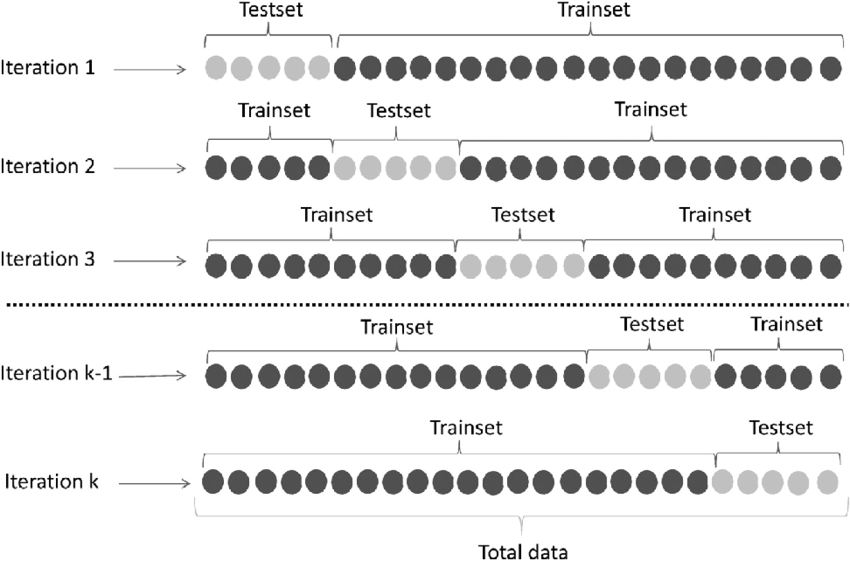
\includegraphics[width=0.9\textwidth]{img/cross.png}
\caption{K-cross validation }
\label{fig:cross}
\end{figure}


\item Bootstrapping : 
\begin{itemize}
\item New datasets are generated by sampling with replacement (uniformly at random) from the original dataset
\item Then train on the bootstrapped dataset and validate on the unselected data
\end{itemize}
\item Jackknife resampling : 
essentially to leave-one-out cross-validation, since leave-one-out is basically sampling without replacement
\end{itemize}


\subsection{Evaluating classification models}\label{eva}
Every model comes with parameters that can modify the model's behavior and performance, evaluation of the model  often comes in the form of a confusion matrix \ref{confu}.
% Please add the following required packages to your document preamble:

% Please add the following required packages to your document preamble:
% \usepackage{multirow}
\begin{table}[]
\centering
\caption{Confusion matrix}
\label{confu}
\begin{tabular}{lllclll}
\cline{3-4}
                                                                                                        & \multicolumn{1}{l|}{}           & \multicolumn{2}{l|}{\textbf{Predicted Class}}                                                                                                                                                            &                               &  &  \\ \cline{3-4}
                                                                                                        & \multicolumn{1}{l|}{}           & \multicolumn{1}{l|}{\textbf{P}}                                                                    & \multicolumn{1}{l|}{\textbf{N}}                                                                     &                               &  &  \\ \cline{1-4}
\multicolumn{1}{|l|}{\multirow{2}{*}{\textbf{\begin{tabular}[c]{@{}l@{}}Actual \\ Class\end{tabular}}}} & \multicolumn{1}{l|}{\textbf{P}} & \multicolumn{1}{l|}{\textbf{\begin{tabular}[c]{@{}l@{}}True Positives\\        (TP)\end{tabular}}} & \multicolumn{1}{l|}{\textbf{\begin{tabular}[c]{@{}l@{}}False Negatives\\        (FN)\end{tabular}}} & \multicolumn{1}{c}{\textbf{}} &  &  \\ \cline{2-4}
\multicolumn{1}{|l|}{}                                                                                  & \multicolumn{1}{l|}{\textbf{N}} & \multicolumn{1}{c|}{\textbf{\begin{tabular}[c]{@{}c@{}}False Positives\\ (FP)\end{tabular}}}       & \multicolumn{1}{c|}{\textbf{\begin{tabular}[c]{@{}c@{}}True Negatives\\ (TN)\end{tabular}}}         & \textbf{}                     &  &  \\ \cline{1-4}
                                                                                                        &                                 & \multicolumn{1}{c}{\textbf{}}                                                                      & \textbf{}                                                                                           & \multicolumn{1}{c}{\textbf{}} &  &  \\
                                                                                                        &                                 & \multicolumn{1}{c}{\textbf{}}                                                                      & \textbf{}                                                                                           & \multicolumn{1}{c}{\textbf{}} &  & 
\end{tabular}
\end{table}


The core values are:
\begin{itemize}
\item True positives (TP): samples classified as positive which were labeled positive
\item True negatives (TN): samples classified as negative which were labeled negative
\item False positives (FP): samples classified as positive which were labeled negative
\item False negatives (FN): samples classified as negative which were labeled positive
\end{itemize}


here is some important quantities we need to know in order to evaluate a model :
\begin{itemize}
\item Recall  also known as True Positive Rate (TPR): $ \frac{TP}{TP+FN}$ 
\item False Positive Rate (FPR): $\frac{TN}{TN+FP}$
\item Positive predictive value:  $\frac{TP}{TP+FP}$ 
\item Negative predictive value: $\frac{TN}{TN+FN}$
\item Precision: How many of the predicted positive samples are correctly predicted   $\frac{\text{TP}}{\text{TP} + \text{FP}}$

\item Accuracy : $\frac{TP+TN}{TP+FP+TN+FN}$

\item The F-score is often introduced as harmonic mean of precision and recall.

$F$-$score= \frac{\text{2} \cdot \text{Precision } \cdot \text{ Recall} }{ \text{Precision} + \text{ Recall}}$



\end{itemize}

\subsubsection{Area under the ROC curve (ROC AUC)}


Receiver Operating Characteristics  ( ROC) is a method that visualizes, organizes and selects models based on  their performance,  this method is for binary classification, but we can adapt it to multi-classification problem  using "OneVsAll" approach, it basically  visualizes the performance of our classifier through all the thresholds, whereas accuracy and F-score  metrics, etc, judge the performance based on particular threshold (usually  0.5) above this cut-off one label is assigned, and below it the other label is assigned. But  looking at all thresholds at once, can give a clear and more honest image of the real performance of our classifier,  since  some models may work best with a different threshold and data sometimes can be biased,   that's when  a dataset has way more or way less of the positive class than there are of the negative class. This imbalance in data can give deceptive and false results if we used accuracy as a metric, to clear the idea more let's say we have a dataset of 100 training example in which it  has 99 example positive and 1 negative example.  The accuracy here can be very deceptive with a value of 99\% so accuracy can't tell much here, the F$\textbf{-}$score can take  into consideration these kind of unbalanced data,  by considering  the true \textbf{positive } rate and the true \textbf{predictive} value  but  it does  not consider all the thresholds of the classifier. However  ROC  is insensitive to bias data ( unbalanced data ) and can run over all thresholds and plots, the  true vs false positive rates, varying the threshold can give us pair of (FPR,TPR) \ref{fig:bias2}.


\begin{figure}[H]
\centering
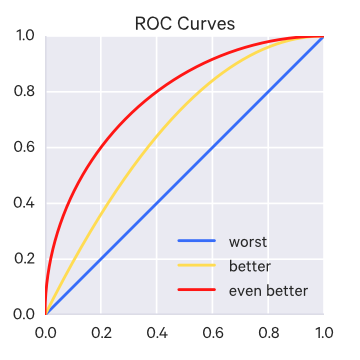
\includegraphics[width=0.5\textwidth]{img/roc.jpg}
\caption{ ROC curve }
\label{fig:bias2}
\end{figure}

The area under the curve (AUC) is used to quantify how good the classifier  is .  The AUC is in fact  the probability that a classifier will rank a randomly chosen positive instance higher than a randomly chosen negative one, (assuming 'positive' ranks higher than 'negative'). Generally, an AUC of above 0.8 is considered "good", an AUC of 0.5 (a straight line) is equivalent to random guessing.
And to generalize this to multi-class, assuming we have a One-vs-All (OvA) classifier, we can either go with the “micro” average or the “macro” average. In “micro averaging,” we’d calculate the performance, e.g., precision and recall, from the individual true positives, true negatives, false positives, and false negatives of the the k-class model:

$$\text{Micro-average of precision} = \frac{TP_{1} \bm{+} TP_{2} \bm{+}....\bm{+}TP_{k}}{TP_{1}\bm{+}TP_{2}\bm{+}....\bm{+}TP_{k}\bm{+}FP_{1}\bm{+}FP_{2}\bm{+}....\bm{+}FP_{k}} 
$$


$$
\text{Micro-average of recall} = \frac{TP_{1}\bm{+}TP_{2}\bm{+}....\bm{+}TP_{k}}{TP_{1}\bm{+}TP_{2}\bm{+}....\bm{+}TP_{k}\bm{+}FN_{1}\bm{+}FN_{2}\bm{+}....\bm{+}FN_{k}} 
$$


And in macro-averaging, we average the performances of each individual class:

$$\text{Macro-average precision} = \frac{PRE_{1}\bm{+}....\bm{+}PRE_{k}}{k} $$
$$\text{Macro-average recall} = \frac{RE_{1}\bm{+}....\bm{+}RE_{k}}{k} $$

Macro-average method can be used when you want to know how the system performs overall across the sets of data. 
On the other hand, micro-average can be a useful measure when your dataset varies in size.

\section{Conclusion:}

In this chapter we have presented in detail some of the most popular classification algorithms in supervised  learning,  such as SVM ( Support Vector Machine ), k-NN (k-Nearest Neighbor ) and in  unsupervised learning the  k-means algorithm, which are going to be used in the classification process after we fed them with the local descriptor, such as SURF / SIFT and feature shape descriptor as of Fourier coefficients, next we studied different methods for selecting  a model using K-fold cross validation, and their astonishing role in maximizing the performance of a classifier by choosing the optimal hyperparameters of a model [\ref{ms}].
Finally we reviewed  how to  assess the performance of a fully trained classifier using area under ROC curve ( ROC AUC ).

In the next chapter we will finally take a look on the techniques used in our HGR system, and we will discuss multiple  project results.    


